\chapter{Estado del arte}

% Descripción de los antecedentes del trabajo.
% Elegir un título apropiado.

\section{Dominio del problema a resolver}

En la actualidad, la digitalización de empresas, administraciones y organismos públicos avanza a ritmo imparable, y la situación excepcional generada por la pandemia de COVID-19 no ha hecho más que afianzar este avance.

Los datos del Índice de Digitalización de la Economía y la Sociedad (DESI) en 2022\cite{desiUE}, índice que monitoriza el rendimiento digital de Europa y el progreso de los países de la Unión Europea en su competitividad digital, muestran que todos los países han progresado en su digitalización. Destaca el hecho de que los países que han empezado en un nivel más bajo de desarrollo digital crecen a un ritmo más rápido, y que numerosos países crecen a un ritmo más elevado del que se les espera, como es el caso de España\cite{desiSpain} (con un 0.7\% más de progreso del esperado).
En concreto, nuestro país es el séptimo con mayor nivel de digitalización según este índice, y el número de personas con competencias digitales básicas es del 64\%, por encima de la media de la UE, del 54\%. Está por encima de la UE también en implementación de la banda ancha fija de al menos 100 Mbps, usuarios de la administración electrónica o pymes con nivel básico de intensidad digital.

%España 2º lugar Índice de Digitalización de la Economía y la Sociedad

%Otras áreas se han modernizado, como todas las empresas. Datos: https://servicioestudiosugt.com/digitalizacion-de-la-empresa-espanola-3-edicion/
A nivel empresarial otros estudios concluyen que la digitalización está más estancada\cite{digitalizacionEmpresaUGT}, debido a una baja inversión en TIC.

%Incluso a nivel de la administración se están impulsando estrategias para avanzar en la digitalización, como España Digital 2026
Por otro lado, a nivel de la administración se están impulsando estrategias para avanzar en la digitalización, como España Digital 2026\cite{espanaDigital2026}, fomentando programas para acelerar la digitalización de pymes (pequeñas y medianas empresas), mejorar la conectividad o desarrollar las competencias digitales en diferentes colectivos.

%Sin embargo, las agrupaciones musicales, que aumentan, siguen sin modernizarse, cuando podrían disfrutar de numerosas ventajas haciendo uso de la tecnología.

Pese a todo esto, algunos sectores de la sociedad aún manifiestan reticencias para proceder a su digitalización, por la falta de herramientas, recursos o ayuda. 
Una de ellas es la que nos ocupa en este trabajo: las asociaciones o agrupaciones musicales. La complejidad de su gestión es suficiente para que los beneficios de la digitalización se puedan manifestar, dada la cantidad de personas que se pueden encontrar en cada una de ellas y la naturaleza de los procesos que siguen, como la programación de ensayos y eventos, la gestión de repertorio o la gestión de miembros.

Por ejemplo, para la correcta planificación de ensayos y eventos, tanto el director como los administradores necesitan conocer con antelación qué músicos tienen pensado asistir y cuáles estarán ausentes. Esto les permitirá saber si se necesita llamar a un músico externo a la agrupación para que participe en un evento, o si es mejor cancelar o aplazar el evento. Para esta tarea, habitualmente el director avisa del evento por un grupo de mensajería a los miembros, y pide que quien no tenga pensado asistir se lo notifique. De este modo se generan varios problemas:

\begin{itemize}
    \item La información sobre qué miembros han notificado su \textit{no asistencia} solo la tiene el director, por lo que si otros administradores quieren conocerla se la tienen que pedir individualmente.
    \item Si algún miembro ha comunicado su ``no asistencia'' a otro administrador, tiene que poner la información en común con la del director, pudiendo dar lugar a discrepancias.
    \item Si el director quiere tener la información de asistencia centralizada, tiene que repasar sus conversaciones con los miembros para elaborar una tabla de asistencia, que tiene que ir actualizando manualmente, con la carga de trabajo que ello supone.
\end{itemize}

Similares problemas se crean para los demás procesos que se llevan a cabo en una agrupación musical.

Es evidente, por tanto, que se necesita una herramienta específica que permita automatizar sus procesos y avanzar en su digitalización para equipararla a la del resto de la sociedad.

Aunque ya existen herramientas como Glissandoo, que se analiza en la sección \ref{subsection:glissandoo}, son de pago, poco personalizables o están poco integradas en el flujo de trabajo actual de las agrupaciones. Es por ello que este trabajo pretende aportar una alternativa libre que solucione estos inconvenientes, de modo que:

\begin{itemize}
    \item Cada agrupación pueda montar su propio servidor con la aplicación, personálizandola y adaptándola a sus necesidades.
    \item Los gastos por uso de la herramienta solo dependan del servidor que use la agrupación, si usa un servidor dedicado.
    \item Sea usable en todas las plataformas en las que se pueda acceder a un navegador web.
    \item Esté integrada en una herramienta de mensajería que ya esté en uso como es \textbf{Telegram}\footnote{\url{https://telegram.org/}}, pero añadiendo funcionalidad específica y automática necesaria para la gestión de la agrupación, eximiendo a los administradores y el director de tareas que se pueden automatizar.
\end{itemize}


% Descripción más detallada del problema, carencias que existen,
% características específicas de los usuarios finales, descripción de
% trabajos previos del cual este es una extensión o de proyectos de 
% investigación en el que se enmarca, etc.

\section{Aplicaciones similares}
% Descripciones, capturas y tabla comparativa
% Alternativas: Glissandoo, Whatsapp

Aunque aún la mayoría de agrupaciones usan Whatsapp como herramienta de comunicación sin usar ningún software más que automatice las tareas, en los últimos tiempos ha surgido otra herramienta que da respuesta a sus necesidades:

\subsection{Glissandoo}\label{subsection:glissandoo}

Glissando\footnote{\url{https://glissandoo.com/}} es un software creado por la empresa Plausible Technologies, con sede en Valencia. En su página web se define como ``un software que nace con el objetivo de profesionalizar, modernizar y digitalizar las instituciones musicales''. Incorpora numerosas funcionalidades para digitalizar instituciones musicales, tal y como pretende este trabajo. Entre ellas se encuentran:

\begin{itemize}
    \item Organización de ensayos y conciertos. Los miembros pueden ver los ensayos y conciertos en la página de inicio.
    \item Previsión de asistencia y pasar lista: para cada ensayo o concierto, el miembro puede seleccionar si tiene prevista su asistencia o no.
    \item Distribución de partituras: en la sección de inicio se puede acceder a un listado de todo el repertorio de los ensayos y conciertos programados, y en cada uno de los ensayos se puede ver el repertorio asociado.
    \item Comunicaciones: los administradores pueden añadir avisos que reciben los miembros, teniendo la capacidad de responder, reaccionar, y adjuntar archivos a los comunicados.
\end{itemize}

Se pueden ver varias capturas de la aplicación en la figura \ref{fig:capturas_glissandoo}.
\begin{figure}[h]
\minipage{0.32\textwidth}
  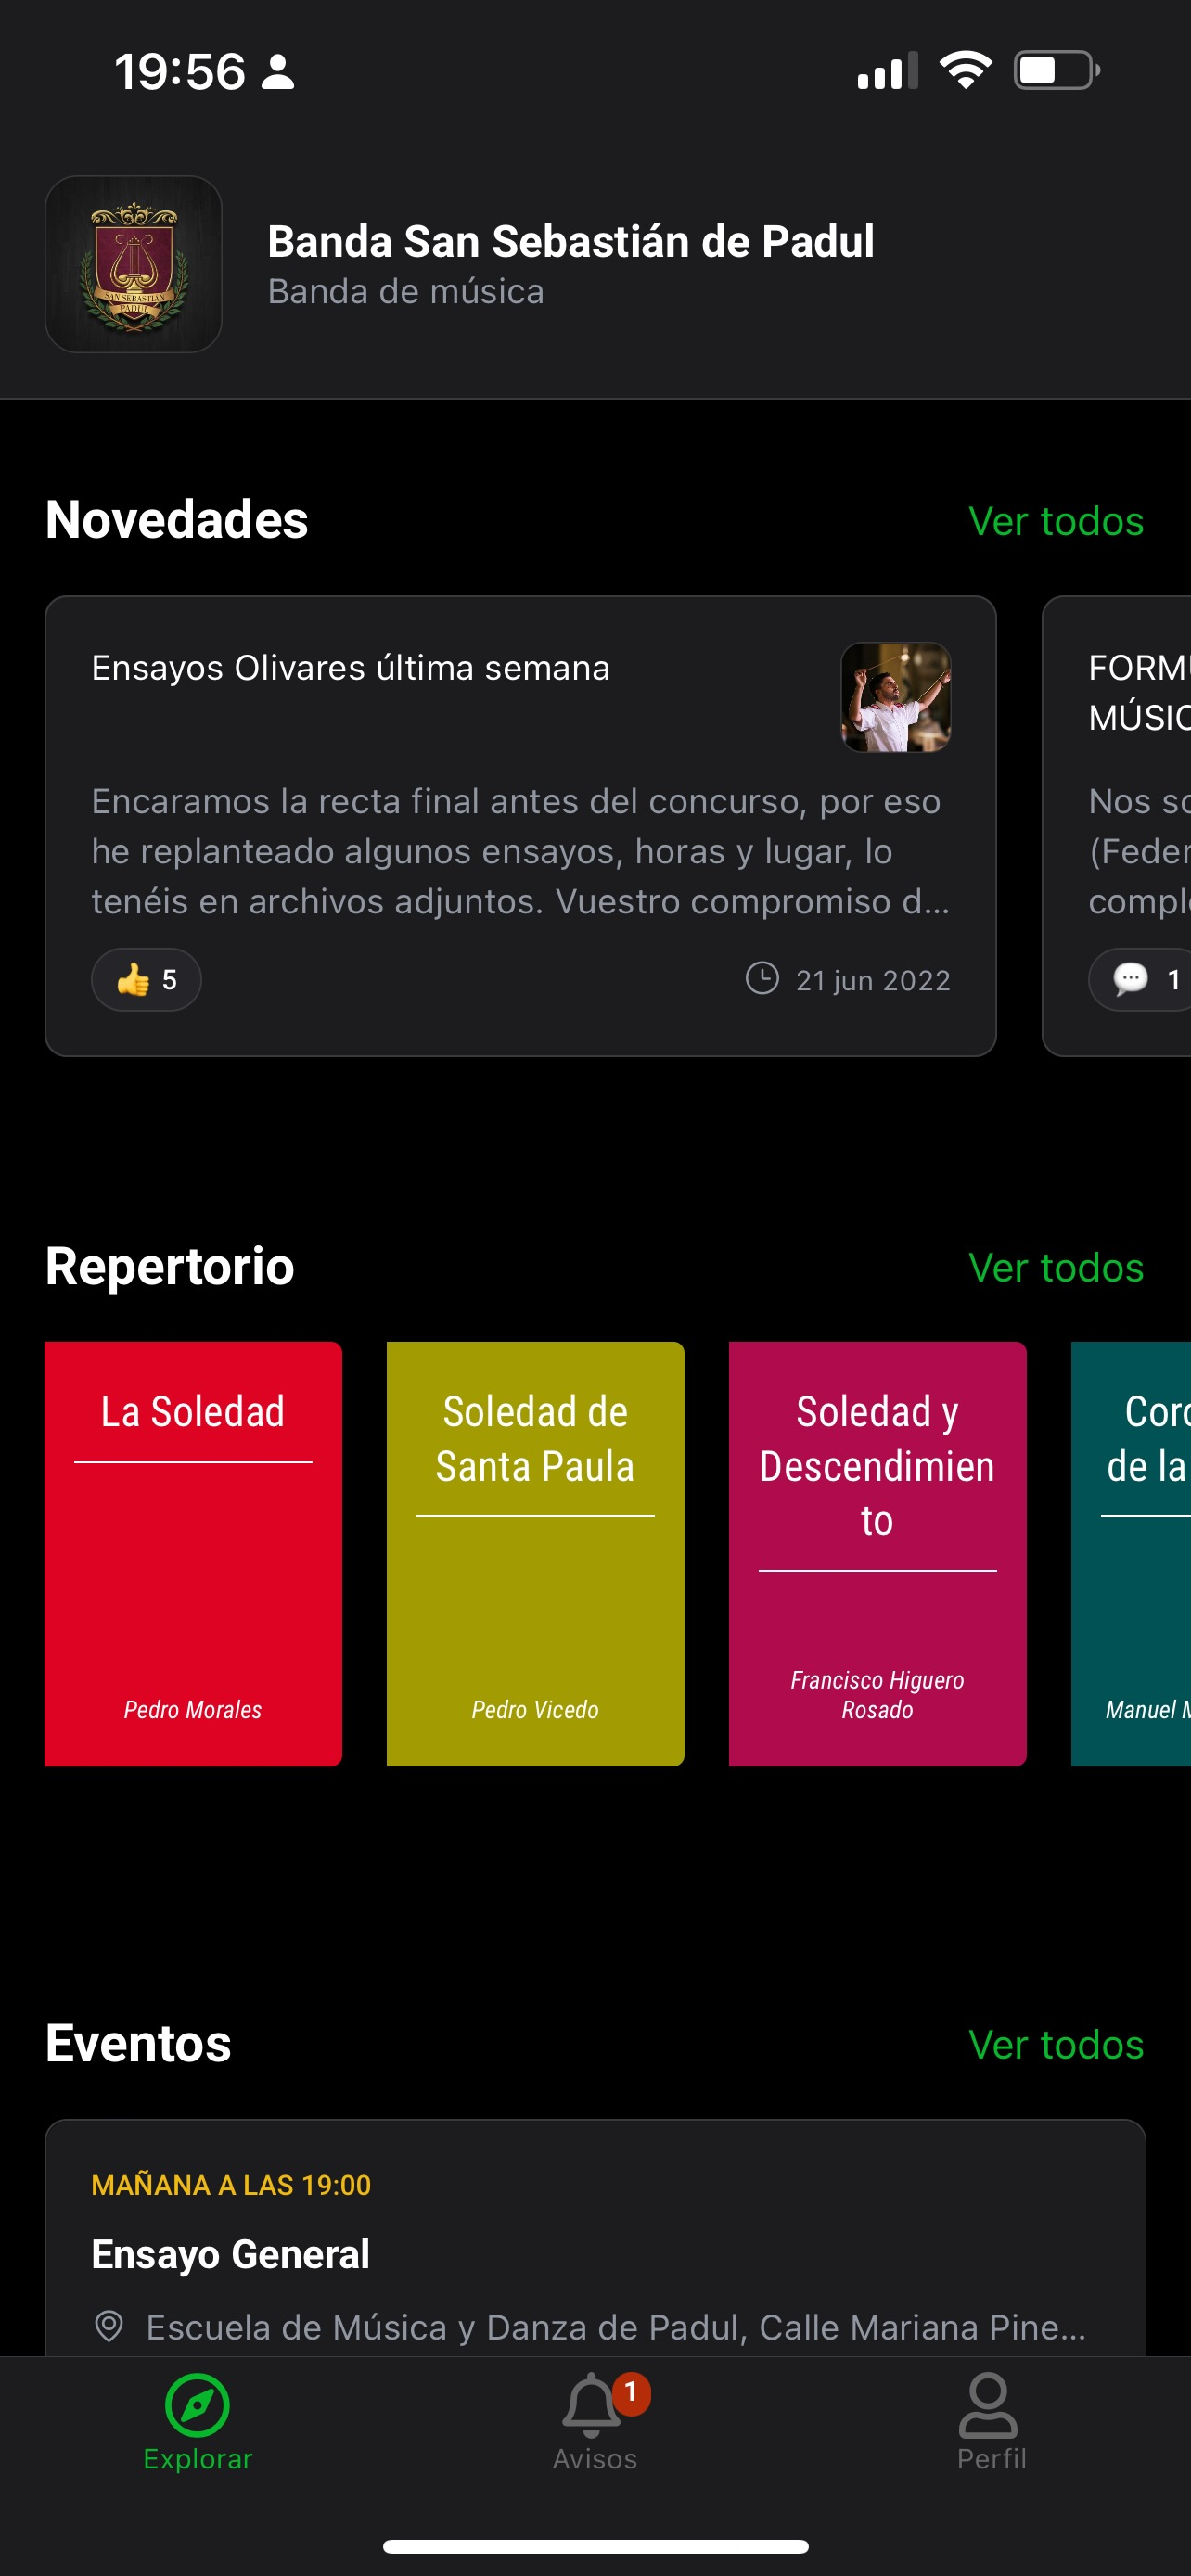
\includegraphics[width=\linewidth]{imagenes/capturas_glissandoo/IMG_0928.jpeg}
\endminipage\hfill
\minipage{0.32\textwidth}
  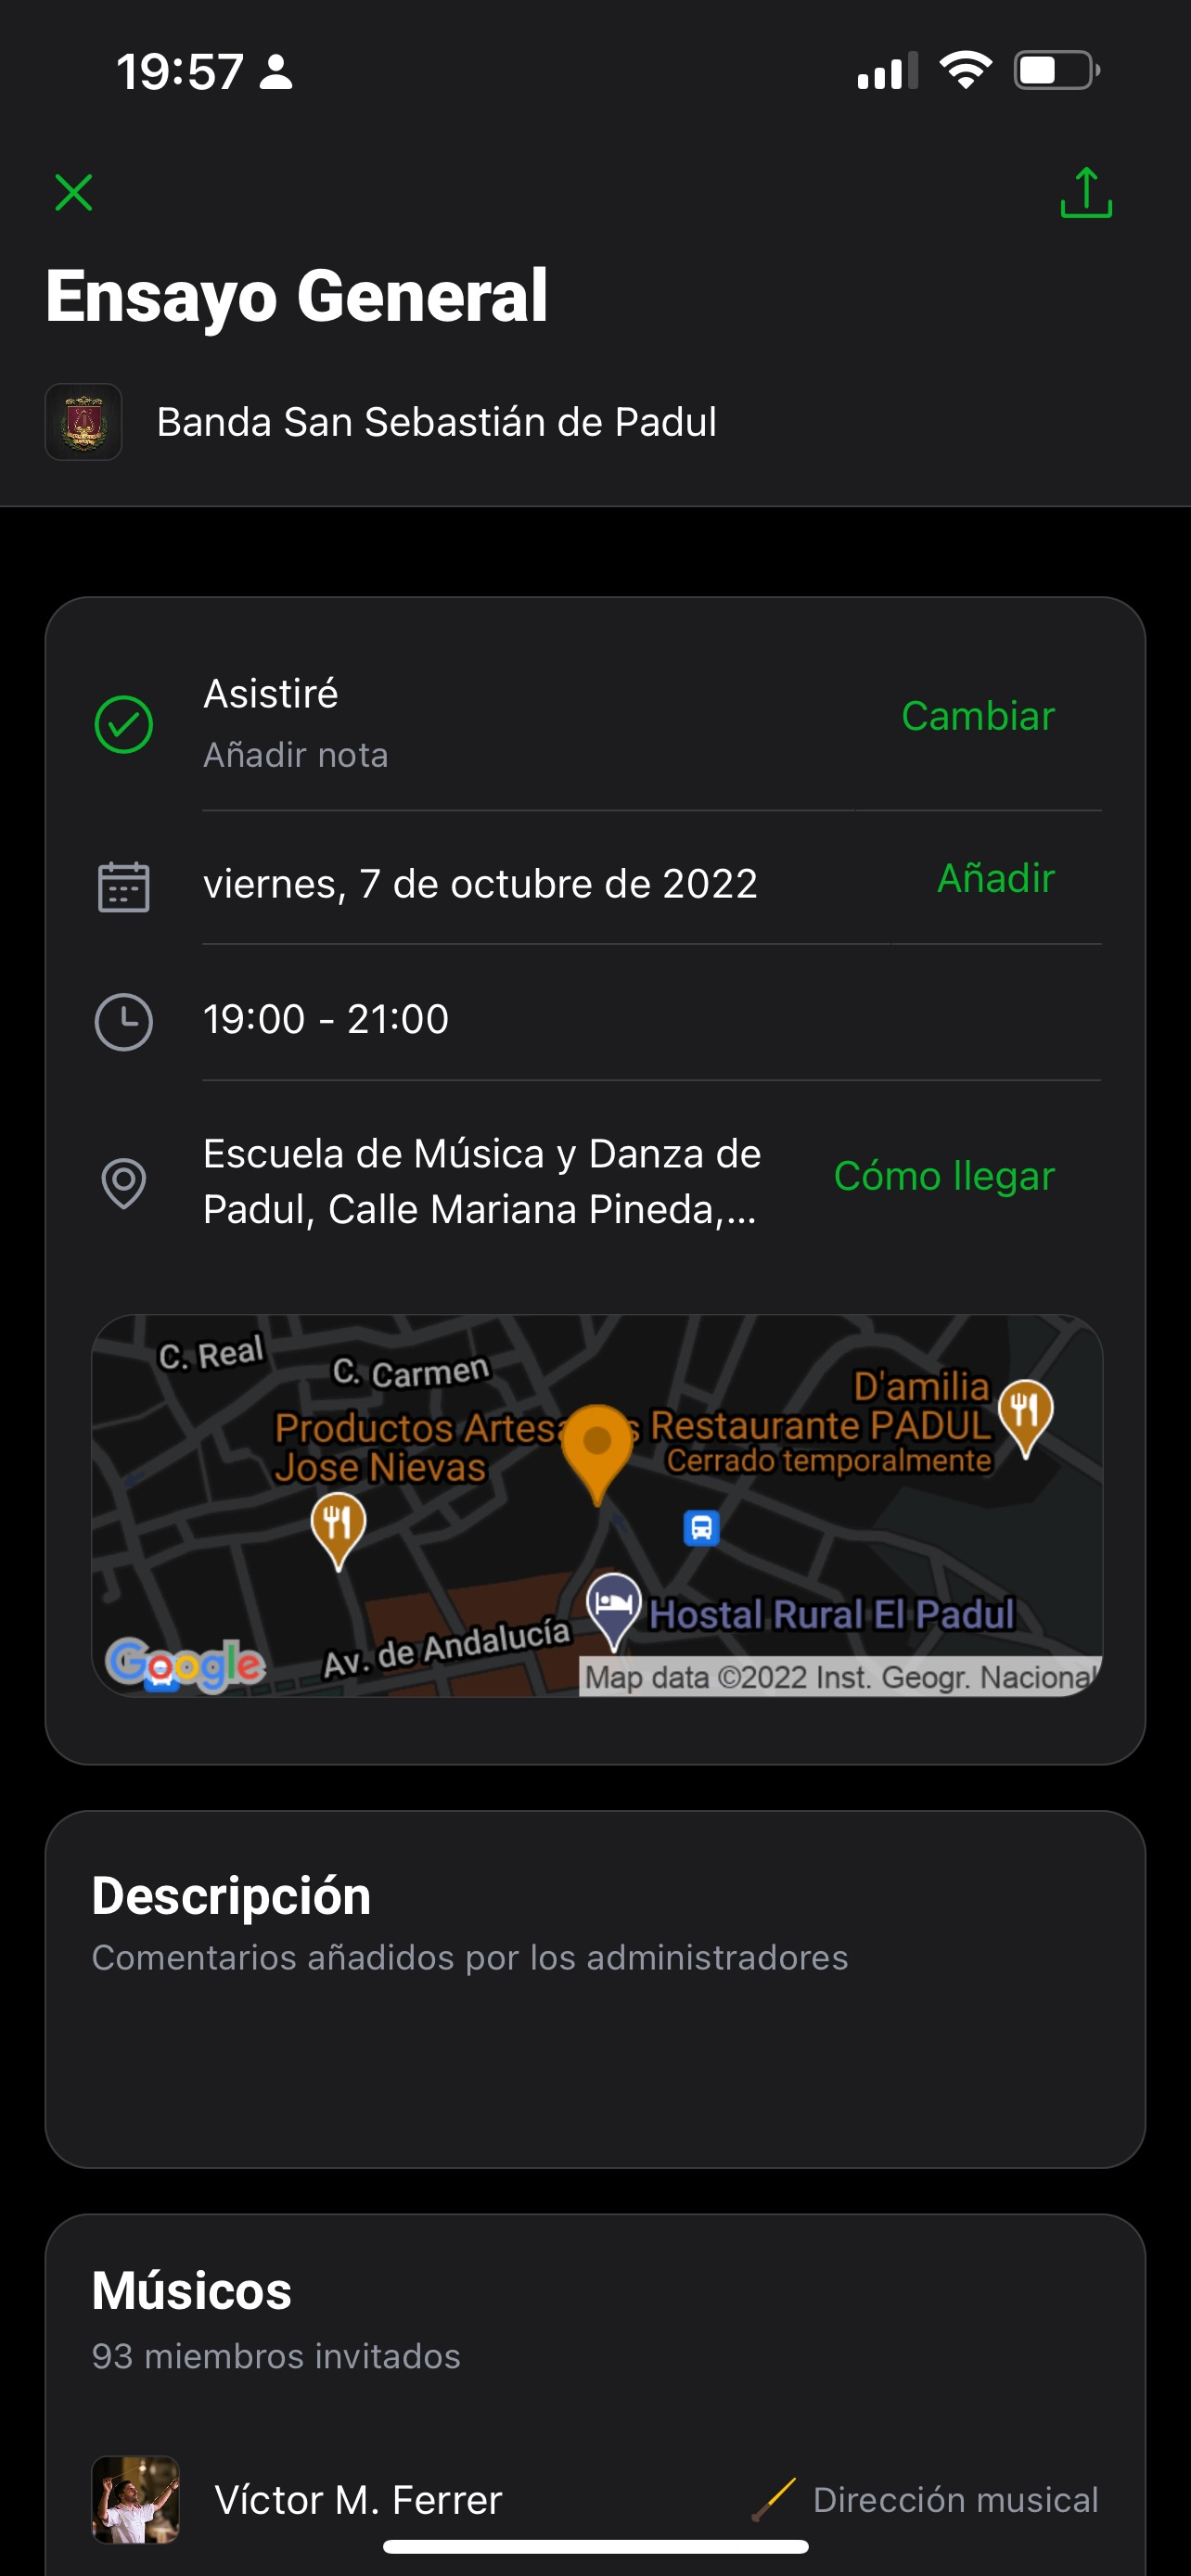
\includegraphics[width=\linewidth]{imagenes/capturas_glissandoo/IMG_0929.jpeg}
\endminipage\hfill
\minipage{0.32\textwidth}
  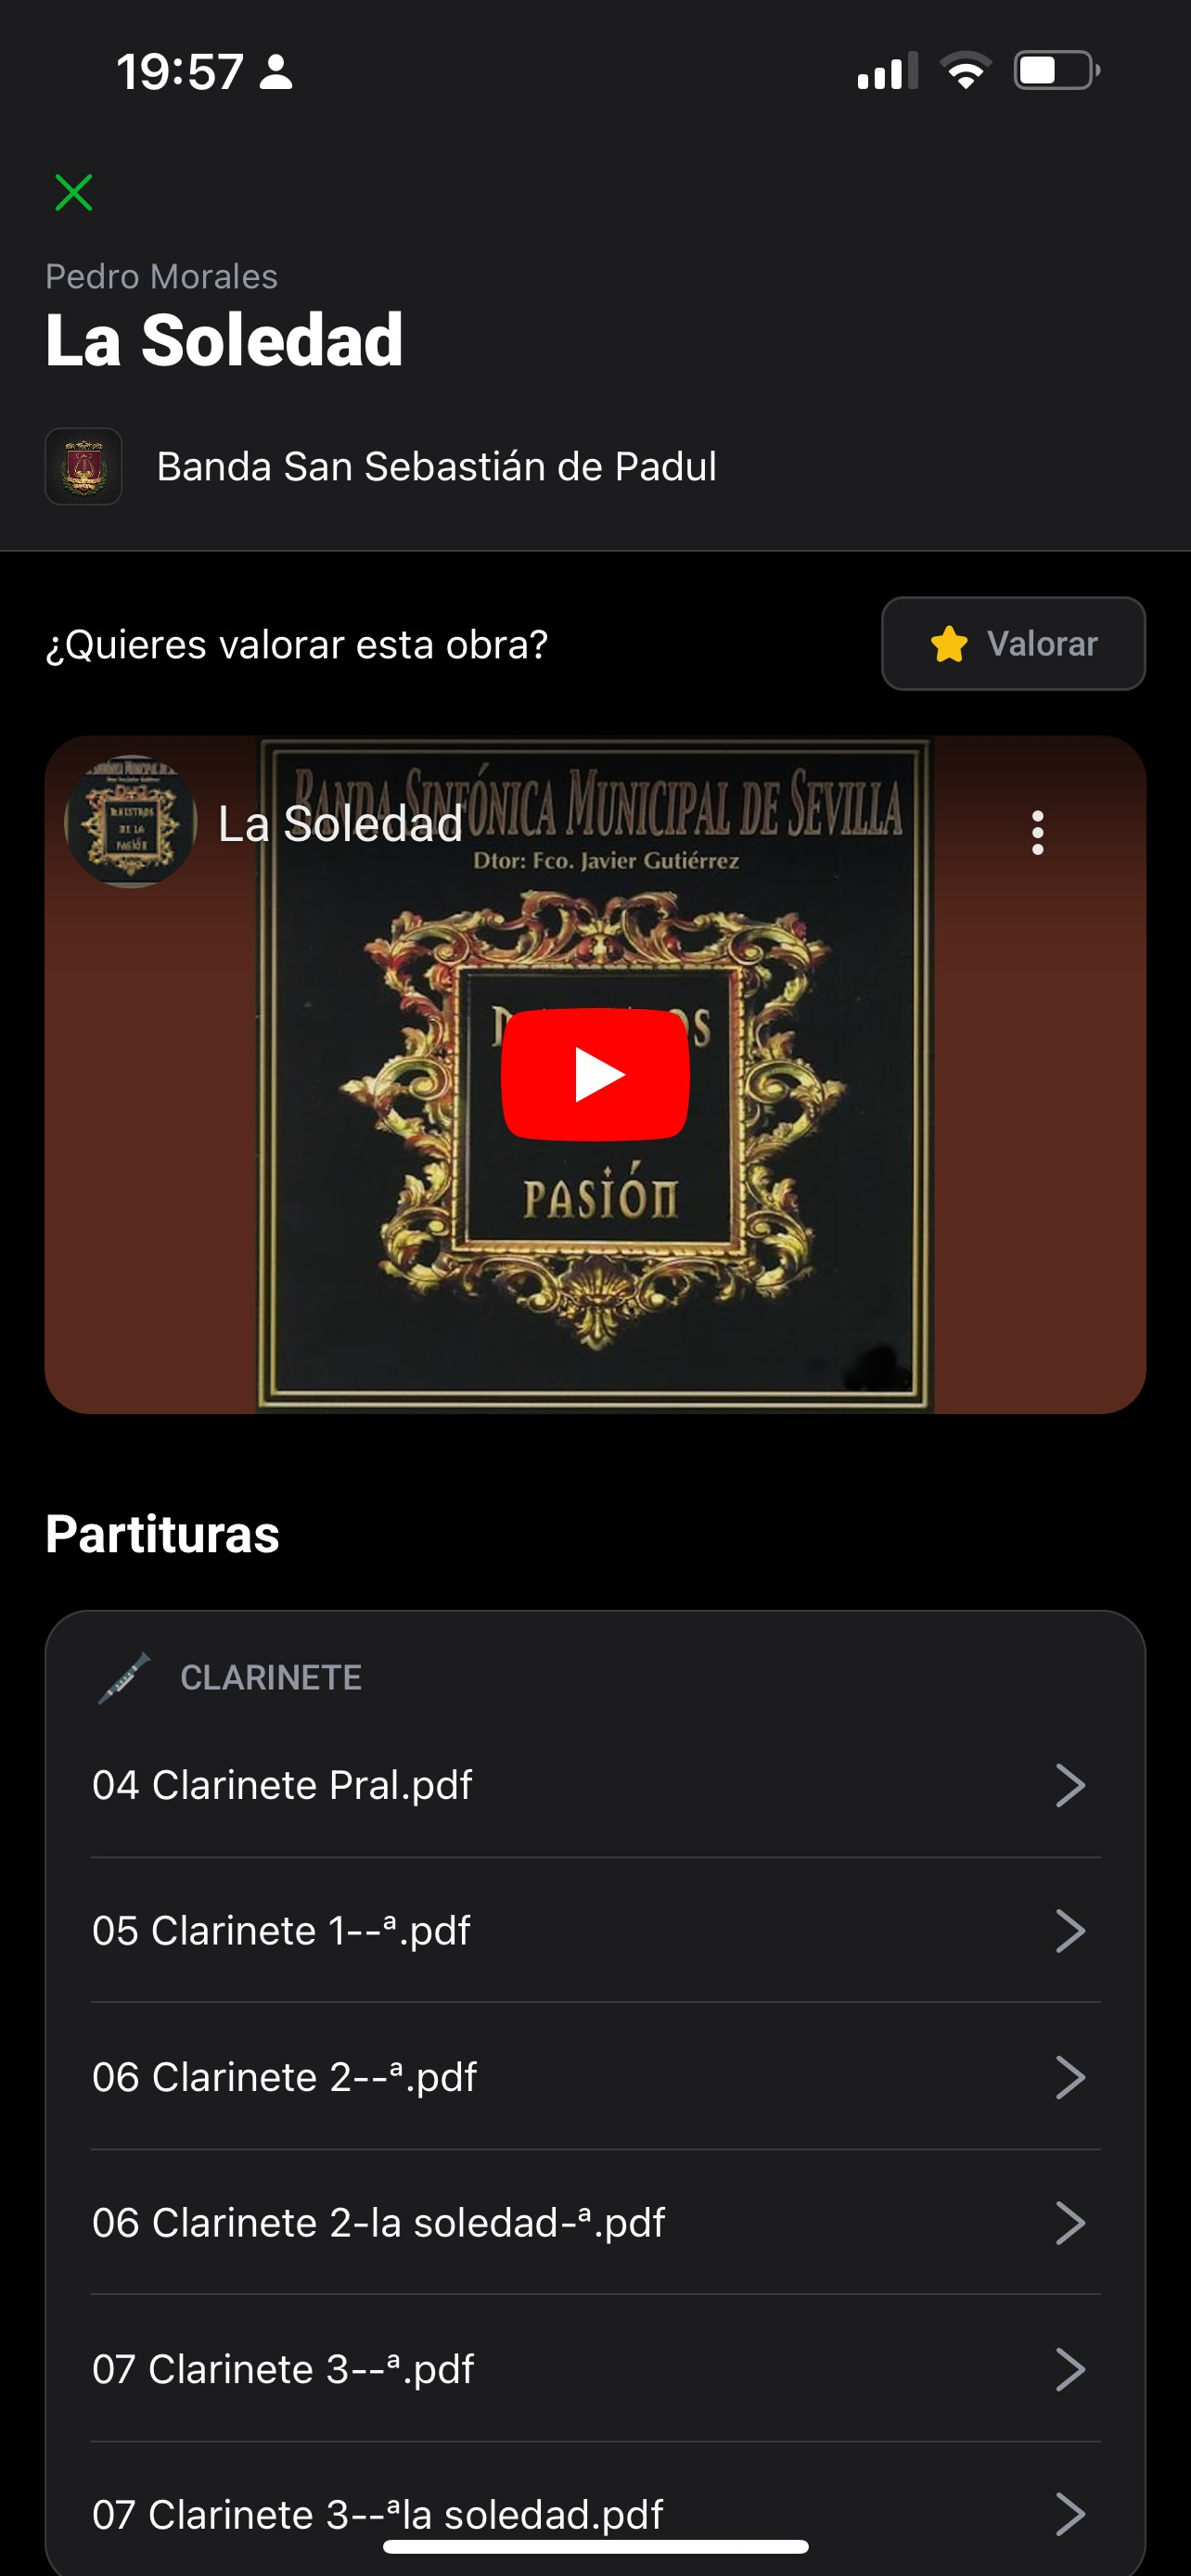
\includegraphics[width=\linewidth]{imagenes/capturas_glissandoo/IMG_0930.jpeg}
\endminipage
\caption{Capturas de la aplicación \textit{Glissandoo}}\label{fig:capturas_glissandoo}
\centering
\end{figure}

Algunas ventajas de esta alternativa son:

\begin{itemize}
    \item Presenta un diseño intuitivo y fácil de usar para todos los usuarios.
    \item Está disponible para las plataformas móviles iOS y Android, ampliamente usadas por los usuarios.
    \item Es gratuita si la agrupación tiene menos de 20 músicos.
    \item Es elaborada en por una empresa valenciana, lo cual da seguridad de que se adaptará a las necesidades de las agrupaciones musicales españolas.
    \item Incorpora un módulo de comunicaciones para poder centralizar todos los procesos de la agrupación en la aplicación, sin dejar los comunicados en otra aplicación de mensajería como WhatsApp.
\end{itemize}

Sin embargo, esta herramienta tiene varias desventajas:

\begin{itemize}
    \item El código es privado, y una agrupación no puede montar su propio servidor con la aplicación en cuestión.
    \item Es de pago para uso en agrupaciones con más de 20 miembros.
    \item Solo se puede usar en móvil, ya que no dispone de versión web ni de escritorio. (Esto ha cambiado durante la realización de este trabajo, ya que han implementado una versión web).
    \item Sigue existiendo duplicidad, ya que aunque los miembros usen esta aplicación, la comunicación bidireccional ocasional entre administradores y miembros de la banda se sigue realizando a través de una herramienta distinta de comunicación no especializada.
\end{itemize}

\subsection{Agregación de servicios no especializados}

Mediante \textit{agregación de servicios no especializados} nos referimos al uso de varias herramientas que no están especializadas para este caso de uso, pero que de cierta forma pueden suplir las necesidades:

\begin{itemize}
    \item Como almacenamiento de partituras, existen servicios como \textbf{Google Drive}\footnote{\url{https://drive.google.com/}}, \textbf{Dropbox}\footnote{\url{https://www.dropbox.com/}} o \textbf{Microsoft OneDrive}\footnote{\url{https://onedrive.live.com/}}.
    \item Para la planificación de eventos y conciertos se puede usar un calendario web como \textbf{Google Calendar}\footnote{\url{https://calendar.google.com/}} o \textbf{Microsoft Outlook}\footnote{\url{https://outlook.live.com/}}.
    \item Para estimar la asistencia se pueden usar herramientas que permiten encuestas de este tipo como \textbf{Doodle}\footnote{\url{https://doodle.com/}}.
    \item Para controlar la asistencia real se puede usar una hoja de cálculo, por ejemplo en \textbf{Google Sheets}\footnote{\url{https://docs.google.com/spreadsheets/}}.
    \item Como medio de comunicación se utiliza otro servicio como \textbf{WhatsApp}\footnote{\url{https://www.whatsapp.com/}} o \textbf{Telegram}\footnote{\url{https://telegram.org/}}.
\end{itemize}

La ventaja de esta aproximación (la mayormente utilizada en la actualidad) es el mayor grado de personalización, ya que los servicios se pueden intercambiar si la funcionalidad o confiabilidad no es la esperada.

No obstante, las desventajas son numerosas, como ya se ha comentado anteriormente:
\begin{itemize}
    \item Gran carga de trabajo para los administradores.
    \item Redundancia de comunicaciones entre los miembros y los administradores.
    \item Muchas de estas herramientas requieren de suscripción \textit{premium} para usar toda la funcionalidad.
\end{itemize}
